\documentclass{beamer} 
\usepackage{amsmath,amsthm}
\usepackage{mathrsfs}
\usepackage{amssymb}
\usepackage[english]{babel}
\usepackage{latexsym}
\usepackage{amsfonts}
\usepackage{graphicx}
\usepackage{float}
\usepackage{graphics}
\usepackage{epsfig}
\usepackage{url}
\usepackage{soul}
\usepackage{listings}
\usepackage{bm}

% \usepackage{minted}


\usetheme{WVU}
\usecolortheme{WVU}
\usepackage{multirow}

\mode<presentation> 

\title[VE401 SU2022 RC week8]{VE401 SU2022 RC week8}

\author[ Shuyu Wu ]{ Shuyu Wu }
\institute[UM-SJTU JI]{UM-SJTU Joint Institute \vspace{.2cm} \\ 
\includegraphics[scale=0.3]{umji_logo.png}\\wushuyu2002@sjtu.edu.cn}
\date[July 2022]{\today}

\begin{document}
\begin{frame} 

\titlepage 

\end{frame} 
\section{Fisher Test} 
\begin{frame}
       \frametitle{Outline}
       \tableofcontents[currentsection]
\end{frame}

\begin{frame}
    \frametitle{Hypotheses and Testing}
    \textbf{definition:} reject or fail to reject statements (hypotheses) based on
    statistical data.\par
    We will make a hypothesis about an unknown parameter $\theta$: $\theta=\theta_0$. The $\theta_0$ here is a given value called null value. The hypothesis is called null hypothesis, denoted as $H_0$\par
    \textbf{example:} given a set of data $X_1, X_2, \dots , X_n$ from a normal distribution $X$,
    \begin{itemize}
        \item (with $\sigma^2=10$ already known) ``$\mu=20$"
        \item (with $\sigma^2$ unknown) ``$\sigma^2 \geq 6$''
        \item (with $\sigma^2$ unknown) ``$\mu\leq 22$''
    \end{itemize}

The basic idea of hypothesis testing is, you first suppose $H_0$ is true, and you find the probability to get the data based on $H_0$. If it's very small(the data is very wierd if $H_0$ holds), then you reject $H_0$.

\end{frame}

\begin{frame}
    \frametitle{P-value}
    The intuitive interpretation of P-value is the probability that $H_0$ gives out such a ``wield'' sample.\par
    For example, $X\sim N(\mu, 5)$ The null hypothesis is $H_0: \mu\leq 26$. We get a sample and the mean is $\overline{x}$. If $\overline{x}\leq 26$, then obviously $H_0$ can't be rejected. If $\overline{x}> 26$, we start to have evidence against $H_0$, and the probability we're interested in is 
    \[P[\overline{X}>\overline{x} | H_0 \text{ is true}]=P[\overline{X}>\overline{x} | \mu\leq 26]\leq P[\overline{X}>\overline{x} | \mu = 26]\]
    The righthand side is the P-value of this hypothesis. It's $1-\Phi(\frac{\overline{x}-\mu}{\sigma/\sqrt{n}})$

\end{frame}

\begin{frame}
    \frametitle{P-value for z-test}

    A hypothesis test on a normal sample, with overall variance known, and the null hypothesis takes one of the three forms:
    \begin{enumerate}
        \item $H_0:\mu\leq\mu_0$
        \item $H_0:\mu\geq\mu_0$
        \item $H_0:\mu=\mu_0$
    \end{enumerate}
    is called a z-test. 1) and 2) are called one-tailed test, 3 is called two-tailed test.\par
    The P-value for 1) is $1-\Phi(\frac{\overline{x}-\mu_0}{\sigma/\sqrt{n}})$.\par
    The P-value for 2) is $1-\Phi(\frac{\mu_0-\overline{x}}{\sigma/\sqrt{n}})$\par
    The P-value for 3) is $2(1-\Phi(\frac{|\overline{x}-\mu_0|}{\sigma/\sqrt{n}}))$

\end{frame}

\begin{frame}
    \frametitle{Conclusion}

    If the P-value(often denoted as $\alpha$) is small, then we have evidence that $H_0$ is false. In this situation, we say $H_0$ is rejected at significance level of $\alpha$. Otherwise, we fails to reject $H_0$.\par
    The threshold is 5\%, however, further study need to be conducted. A small P-value doesn't necessarily means that $H_0$ is indeed false.

\end{frame}



\begin{frame}
    \frametitle{Disadvantage of Fisher test}

    $a\rightarrow b,P[b] \text{ is low}$, doesn't mean $P[a]$ is low.\par
    \vspace*{0.3cm}
    Also, it seems that when n is big enough, the P-value of two-tailed test will always be small.

\end{frame}

\begin{frame}
    \frametitle{ex 8.1}
    $X\sim(\mu, 5^2)$ and $H_0: \mu=10$. Take 10 sample and we find $\overline{x}=11$. What's the P-value?\par
    \vspace*{0.3cm}

    The test statistic is $Z=\frac{\overline{X}-\mu_0}{\sigma/\sqrt{n}}=\frac{\overline{X}-10}{5/\sqrt{10}}$. Now the experimental value is $\frac{11-10}{5/\sqrt{10}}=0.632$. $\alpha=0.264*2=0.528$ This is large, so we fail to reject $H_0$.
    

\end{frame}

\section{Neyman-Pearson Decision Theory}
\begin{frame}
    \frametitle{Outline}
    \tableofcontents[currentsection]
\end{frame}
\begin{frame}
    \frametitle{Setup}

    We now need two hypotheses. One is the null hypothesis $H_0$, the other is $H_1$, called alternative
    hypothesis. In NPDT, we aim at finding the correct hypothesis, rather than only against $H_0$.\par
    Example: $H_0: \mu=40;\; H_1: |\mu-40|\geq 1$\par
    Two indicator: 
    \begin{itemize}
        \item $\alpha$, called the significance level or error of the I kind, means $P[\text{reject }H_0|H_0 \text{ is true}]$.
        \item $\beta$, called error of the II kind, means $P[\text{accept }H_0|H_1 \text{ is true}]$. $1-\beta$ is called power.
    \end{itemize}
    

\end{frame}

\begin{frame}
    \frametitle{Critical Region}
    The critical region means, if the statistic falls into this region, the $H_0$ is rejected at the significance level of $\alpha$. The critical region must be fixed before data are obtained.
    \begin{enumerate}
        \item $H_0:\mu=\mu_0$, critical region is $\overline{x}\neq \mu_0\pm z_{\alpha/2}\frac{\sigma}{\sqrt{n}}$
        \item $H_0:\mu\leq\mu_0$, critical region is $\overline{x}> \mu_0+ z_{\alpha}\frac{\sigma}{\sqrt{n}}$
        \item $H_0:\mu\geq\mu_0$, critical region is $\overline{x}< \mu_0- z_{\alpha}\frac{\sigma}{\sqrt{n}}$
    \end{enumerate}
    
\end{frame}

\begin{frame}
    \frametitle{$\beta$ and sample size}
    $\beta$ can be controlled by increasing sample size $n$. For a two-tailed null hypothesis, if we need to get a desired $\beta$, we need $n\geq\frac{(z_{\alpha/2}+{z_{\beta}})^2\sigma^2}{\delta^2}$.\par
    Here $\delta$ is the interval between $H_0$ and $H_1$.
    
    

\end{frame}

\begin{frame}
    \frametitle{ex 8.2}
    $H_0: \mu=40;\; H_1: |\mu-40|\geq 1$. We already know sample variance is 4. Now we get a set of 40 samples with $\overline{x}=40.3$. Set $\alpha=0.05$.\par
    Is $H_0$ rejected? What's $\beta$?\par
    \vspace*{0.3cm}

\end{frame}

\begin{frame}
    \frametitle{ex 8.2 answer}

    $z_{\alpha/2}\frac{\sigma}{\sqrt{n}}=1.96*2/\sqrt{40}=0.619$, so critical region is $\mu\neq 40\pm 0.619$. $\overline{x}$ is not in the critical region, so $H_0$ is accepted.\par
    Now calculate $\beta$. $n=\frac{(z_{\alpha/2}+{z_{\beta}})^2\sigma^2}{\delta^2}$, so $40=(1.96+z_{\beta})^2*2$, $z_{\beta}=2.51$, $\beta=0.006$.

\end{frame}

\begin{frame}
    \frametitle{OC Curve}
    OC Curve is a plot of actual $\mu$ vs. $P[H_0 \text{ is accepted}]$.\par
    For a two-tailed z-test, when $\mu=\mu_0$, the value is $1-\alpha$ since there's $\alpha$ probability that we reject $H_0$ when $H_0$ is correct.\par
    When $\mu$ is the bounded value of $H_1$, the value is $\beta$ since now $H_1$ is true.\par
    Notice that for different n, the curve is different.\par
    In practice our OC curve is a plot of $d$ vs $P[H_0 \text{ is accepted}]$. $d:=\frac{\mu-\mu_0}{\sigma}$.
    This is the OC curve of two-tailed z-test.
    \begin{figure}[H]
        \centering
        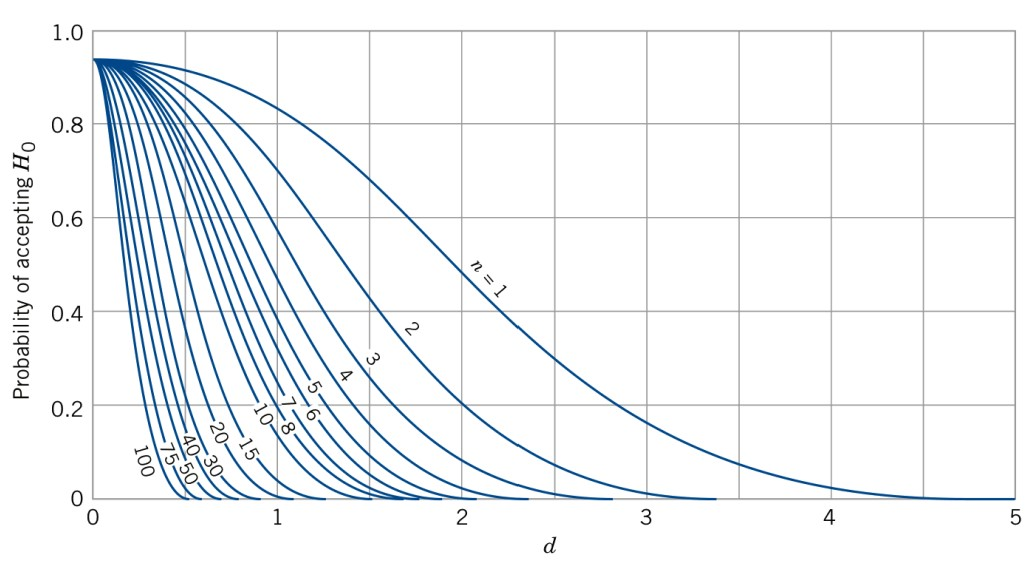
\includegraphics[width=0.45\textwidth,height=0.2\textwidth]{z_oc_2tail.jpg}
        \caption{two-tailed z-test}
    \end{figure}\par

\end{frame}

\section{Null Hypothesis Significance Testing}
\begin{frame}
    \frametitle{Outline}
    \tableofcontents[currentsection]
\end{frame}

\begin{frame}
    \frametitle{Null Hypothesis Significance Testing(NHST)}
    Many textbooks use NHST. It's a mixture of fisher test and NPDT.\par
    We set a significance level $\alpha$, and calculate the critical region. The form is similar to NPDT, but its essence is closer to fisher test. Many people think when $H_0$ is rejected, they can definitely get the result, which is wrong.\par
    \vspace*{0.3cm}
    In conclusion, you do not need to use NHST.
    

\end{frame}

\section{Single Sample Tests for the Mean and Variance}
\begin{frame}
    \frametitle{Outline}
    \tableofcontents[currentsection]
    

\end{frame}

\begin{frame}
    \frametitle{Test Statistic}
    When we suppose $H_0$ is true, some statistic will follow a certain distribution. We call such statistic a \textbf{test statistic}. For example, in z-test, $Z=\frac{\overline{X}-\mu_0}{\sigma/\sqrt{n}}$ is the test statistic, which should follow a standard normal distribution. If the sample value is far from 0, then $H_0$ is rejected.\par
    In the following hypothesis testing, we always use this kind of method.

\end{frame}

\begin{frame}
    \frametitle{T-test}
    For the null hypothesis $\mu=\mu_0$ \par
    Now suppose we don't know the overall variance $\sigma^2$. We need to use $S^2$ instead. And the test statistic is $T_{n-1}=\frac{\overline{X}-\mu_0}{S/\sqrt{n}}$, which follows a student-T distribution.\par
    Then, the critical region at significance level $\alpha$ is given by $|T_{n-1}|>t_{\alpha/2,n-1}$, or $\overline{x}\neq \mu_0\pm t_{\alpha/2,n-1}\frac{S}{\sqrt{n}}$\par
    \vspace*{0.3cm}
    For $H_0: \mu\leq \mu_0$, the critical region at significance level $\alpha$ is given by $T_{n-1}>t_{\alpha,n-1}$, or $\overline{x}> \mu_0+ t_{\alpha,n-1}\frac{S}{\sqrt{n}}$\par
    \vspace*{0.3cm}
    For $H_0: \mu\geq \mu_0$, the critical region at significance level $\alpha$ is given by $T_{n-1}<-t_{\alpha,n-1}$, or $\overline{x}< \mu_0- t_{\alpha,n-1}\frac{S}{\sqrt{n}}$\par

\end{frame}

\begin{frame}
    \frametitle{T-test: $\beta$}

    To complete a NPDT, we need to figure out the power. Now there's no formula(we need non-central T -distributions), so we need to rely on OC-curve directly.\par
    In the calculation of $d$, the $\sigma$ can be approximated by $S$.\par
    Please figure out if it's one-tail or two tail before using the OC curve. Resources of OC curves are avaliable on canvas.

\end{frame}

\begin{frame}
    \frametitle{Chi-squared Test}

    Chi-squared test is used to test the hypotheses that are related to variance or standard deviation.\par
    The test statistic is $\chi_{n-1}^2=\frac{(n-1)S^2}{\sigma_0^2}$. At significance level $\alpha$, the critical region is:
    \begin{itemize}
        \item $H_0: \sigma=\sigma_0$: $\chi_{n-1}^2>\chi_{\alpha/2,n-1}^2$ or $\chi_{n-1}^2<\chi_{1-\alpha/2,n-1}^2$
        \item $H_0: \sigma\leq \sigma_0$: $\chi_{n-1}^2>\chi_{\alpha,n-1}^2$ 
        \item $H_0: \sigma\geq \sigma_0$: $\chi_{n-1}^2<\chi_{1-\alpha,n-1}^2$
    \end{itemize}
    For $\beta$, you can still read it from the OC curve. Notice that $\lambda=\frac{\sigma}{\sigma_0}$

\end{frame}

\section{Non-Parametric Single Sample Tests for the Median}

\begin{frame}
    \frametitle{Outline}
    \tableofcontents[currentsection]
\end{frame}

\begin{frame}
    \frametitle{Non-Parametric Statistics}

    Previous method assume samples to be i.i.d normal sample. However, the sample can be neither independent nor following a normal distribution.\par
    In this kind of situation, we focus on median and IQR instead of mean and variance. These kind of statistics are called non-parametric statistic. The method that do not assume normal distribution or independence is called non-parametric test.

\end{frame}

\begin{frame}
    \frametitle{Sign Test for Median}

    The null hypothesis is of these kinds: 
    \begin{itemize}
        \item $H_0: M=M_0$
        \item $H_0: M\leq M_0$
        \item $H_0: M\geq M_0$
    \end{itemize}
    $M$ is the median. Now given a sample $X_1, X_2,\dots , X_n$, we want to figure out whether $H_0$ should be rejected.\par
    Set $Q_{+}$ be the number of the sample that is greater than $M$, $Q_{-}$ be the number of the sample that is smaller than $M$. We have 
    \[P[Q_{-}\leq k]=P[Q_{+}\leq k]=\frac{1}{2^n}\sum\limits_{x=0}^{k} \binom{n}{x}\]

\end{frame}

\begin{frame}
    \frametitle{P-value}

    For null hypothesis
    \begin{itemize}
        \item $H_0: M\leq M_0$ The P value is $P[Q_{-}\leq k|M=M_0]$
        \item $H_0: M\geq M_0$ The P value is $P[Q_{+}\leq k|M=M_0]$
        \item $H_0: M= M_0$ The P value is $2*P[min\{Q_{+},Q_{-}\}\leq k|M=M_0]$
    \end{itemize}
    k is the corresponding count in the sample.\par
    When the P-value is below the significance level $\alpha$, $H_0$ is rejected.

\end{frame}

\begin{frame}
    \frametitle{Wilcoxon Signed Rank Test}

    It only apply to symmetric distribution. That is to say, $f_{X-a}(x)=f_{a-X}(x)$, or $f_{X}(a-x)=f_{X}(a+x)$. (the version on the slide seems to be wrong).\par
    \vspace*{0.3cm}
    Then, sort the sample data by the distance to the $M_0$, and give a rank to each of them. The sample with smallest get 1, followed by 2,3,..., n.\par
    Set $W_{+}$ to be the positive rank(i.e., the sum of all the sample that is bigger than $M_0$). $W_{-}$ to be the negative rank.\par

    Test statistic: $W$ will follow a normal distribution with expectation $\frac{n(n+1)}{4}$, variance $\frac{n(n+1)(2n+1)}{24}$. And for each group of t ties, the variance is reduced by $\frac{t^3-t}{48}$\par
    Finally, do the same thing as z-test.

\end{frame}

\begin{frame}
    \frametitle{TL;DR}

    Use mathematica or matlab to perform the test!\par
    

\end{frame}

\section{Inferences on Proportions}
\begin{frame}
    \frametitle{Outline}
    \tableofcontents[currentsection]
\end{frame}

\begin{frame}
    \frametitle{Estimating Proportions}
    $X$ follows a 0-1 (or Bernoulli) distribution with parameter $p$. We have a set of n i.i.d sample $X_1, X_2, \dots , X_n$.\par
    Then $\hat{p}=\frac{1}{n}\sum\limits_{i=1}^{n}X_i$. \par
    By central limit theorem, a $100(1-\alpha)\%$ two-side confidence interval for p is roughly given by 
    \[\hat{p}\pm z_{\alpha/2}\sqrt{\frac{\hat{p}(1-\hat{p})}{n}}\]
    
    To ensure $|\hat{p}-p|\leq d$ under this confidence level, if we do not know anything about $\hat{p}$, we have $n=\frac{z_{\alpha/2}^2}{4d}$

\end{frame}

\section{Extra topic and Q\&A}
\begin{frame}
    \frametitle{Outline}
    \tableofcontents[currentsection]
\end{frame}

\begin{frame}
    \frametitle{Extra topic}
    \begin{itemize}
        \item P-hacking and the fraud in research
        
    \end{itemize}
    

\end{frame}


\begin{frame}
    \frametitle{Q\&A}
    
    Feel free to ask if you have any questions.\par
    
    
    
\end{frame}

\end{document} 